\chapter{Caracterización y modelado de la planta} \chapterlabel{Informe/3-CaracterizacionElectroiman} \label{cap:CaracterizacionElectroiman}

En este capítulo se realiza un modelado físico del sistema para encontrar una expresión de la fuerza magnética ejercida en función de la variable de control. Además, se detallan las características constructivas que posee el electroimán y las mediciones realizadas. Luego, se realiza el modelo de estados de la planta y se obtienen otros parámetros relevantes para el diseño del sistema de control.

\section{Modelado matemático del electroimán}

En esta sección se desarrollan las ecuaciones matemáticas que describen el funcionamiento del electroimán. Para ello se analizan las fuerzas que se aplican a la pieza móvil y la naturaleza de las mismas.

Como se mencionó previamente, para el desarrollo del proyecto se utiliza un electroimán compuesto por dos piezas: una con forma de “E” y otra con forma de “I”. Al analizar esta última, se pueden observar dos fuerzas opuestas en el eje vertical como se muestra en la figura \ref{fig:img_Esquema-del-producto}. Una es la fuerza magnética generada por el electroimán, y la otra es la generada por la acción de la gravedad sobre la masa del objeto.  

%\noindent Se puede modelar el sistema como un objeto de masa puntual que es sometido a dos fuerzas opuestas en el eje vertical de la figura \ref{fig:img_modelado-fisico}: la de su propio peso hacia abajo, y una fuerza realizada por el electroimán en sentido contrario. \colorbox{red}{MARCAR Yo EN LA IMAGEN}

\noindent La fuerza correspondiente al peso del objeto es $P=M*g$, donde $M$ es la masa en kg y $g$ es la aceleración de la gravedad en $m/s^2$. Para que se mantenga levitando en estado de equilibrio, el electroimán debe generar una fuerza magnética ($F_{m}$) de igual módulo pero sentido contrario.

\noindent La fuerza de atracción entre las dos piezas se logra al hacer circular un flujo magnético entre ellas. Este es generado por la corriente en el bobinado del electroimán.

\noindent En el núcleo se genera una fuerza magnetomotriz ($F_{mm}$) debido a la corriente del bobinado, y es la responsable de la circulación del flujo magnético. La ecuación \ref{eq_fuerza-magnetomotriz} da una relación de estos parámetros.	


%\noindent Para que haya una fuerza que atraiga la pieza I hacia la E, se necesita que entre estas circule un flujo magnético. Este es generado a partir de una fuerza magnetomotriz ($F_{mm}$), cuyo módulo está dado por la ecuación \ref{eq_fuerza-magnetomotriz}.

%\noindent Al haber una corriente circulando por el bobinado, se genera una fuerza magnetomotriz en el núcleo del electroimán, la que a su vez provoca la circulación de un flujo magnético entre las dos piezas. De esta manera se genera una fuerza magnética que las atrae.

%La fuerza magnética e generada a partir del flujo magnético Para generar un flujo magnético se necesita una fuerza magnetomotriz.

%que es generada por la circulación de un flujo magnético entre las dos piezas. La fuerza magnetomotriz ($F_{mm}$) es la que hace posible el flujo de energía. Esta es generada por la corriente que circula en el bobinado. Su módulo está dado por la ecuación \ref{eq_fuerza-magnetomotriz}.

\begin{equation} \label{eq_fuerza-magnetomotriz}
	\abs{F_{mm}}=N*i=R_{m}*\phi	
\end{equation}

\noindent Donde: 
\begin{itemize}
	\item $F_{mm}$: fuerza magnetomotriz.
	\item N: cantidad de vueltas del bobinado.
	\item i: corriente que circula por el bobinado.
	\item $R_{m}$: reluctancia del circuito magnético.
	\item $\phi$: flujo magnético.
\end{itemize}


\noindent Por otro lado, la inductancia del bobinado ($L$) está dada por la ecuación \ref{eq_inductancia_flujo}.

\begin{equation} \label{eq_inductancia_flujo}
	L*i=N*\phi
\end{equation}

\subsection{Modelado de inductancia del electroimán}

Las dos piezas del electroimán, junto con el entrehierro que las separa, conforman un circuito magnético. Debido a la alta permeabilidad del material ($\mu_{r}$) por el que están hechas, el flujo magnético circula dentro del volumen del núcleo y solo lo hace por el aire cuando atraviesa la separación de las piezas.

Debido a la simetría del electroimán, el flujo magnético total generado en su rama central se divide en dos para circular por cada rama lateral como se observa en la figura \ref{fig:img_flujo}.

\begin{figure}[H]
	\centering
	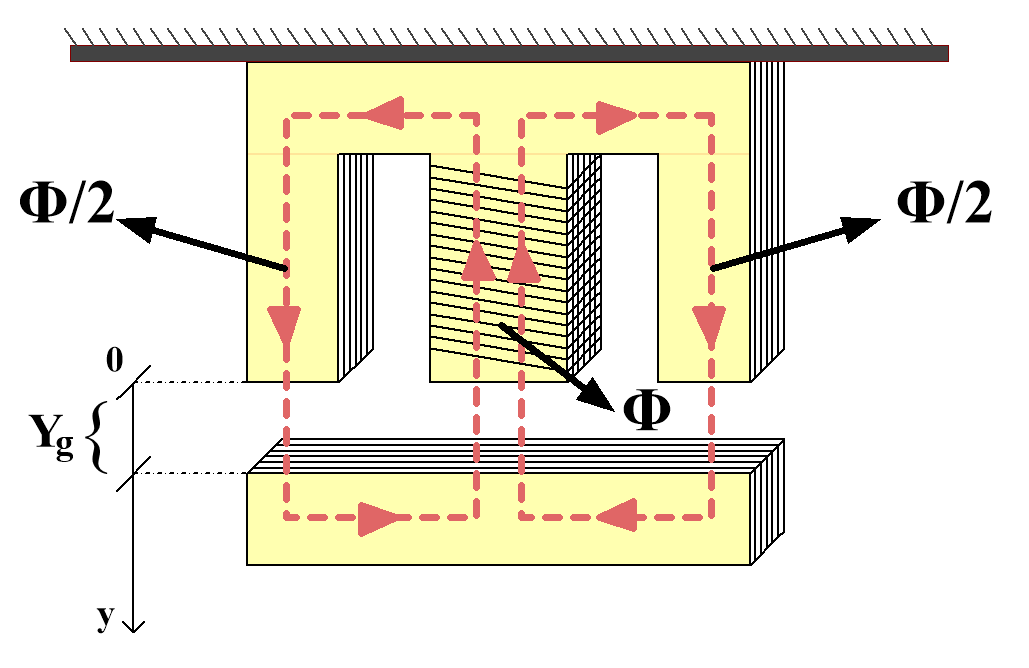
\includegraphics[scale=0.5]{flujo.png}
	\caption{Circulación del flujo magnético a través del electroimán.}
	\label{fig:img_flujo}
\end{figure}

\noindent Para encontrar una expresión de la inductancia del electroimán se utiliza de la Ley de Ampere mostrada en la ecuación \ref{eq_ampere}. Esta relaciona la magnitud de la fuerza magnetomotriz con la integral de camino de la intensidad de campo magnético ($H$).

\begin{equation} \label{eq_ampere}
	F_{mm}=\oint{H*dl}=N*i
\end{equation}

\noindent La intensidad de campo magnético depende del medio en el que se propague el flujo magnético. Por lo tanto, en el núcleo será distinta que en el entrehierro. Por ello es conveniente utilizar la densidad de flujo magnético (B), cuya relación es $H=\frac{B}{\mu}$. De esta forma, se puede separar la porción de integral dentro del material ferromagnético y en el entrehierro. Entonces la fuerza magnetomotriz queda:

\begin{equation} 
	F_{mm}=\oint{\frac{B}{\mu_{o}}*dl}+\oint{\frac{B}{\mu_{r}}*dl}=N*i
\end{equation}

\noindent Para cada camino que recorre el flujo magnético, la intensidad de campo magnético es constante. Por lo tanto, se resuelven las integrales:

\begin{equation}\label{eq_fuerza-mm}
	F_{mm}=\frac{B}{\mu_{r}}*l_{m}+\frac{B}{\mu_{o}}*l_{A}=N*i
\end{equation}

Donde:
\begin{itemize}
	\item $l_{m}$: longitud del circuito magnético dentro del electroimán.
	\item $l_{A}$: longitud del circuito magnético en el entrehierro.
	\item $\mu_{o}$: permeabilidad magnética del vacio ($4 \pi * 10^{-7}\:H/m$).
	\item $\mu_{r}$: permeabilidad magnética relativa del material del electroimán. Su valor es aproximadamente igual a $4000 * \mu_{o}$.
	
\end{itemize}

\noindent Debido a la definición de  densidad de flujo magnético se tiene:

\begin{equation}\label{eq_definicion-camp-magn}
	B=\frac{\phi}{A}
\end{equation}

En la expresión \ref{eq_definicion-camp-magn} el área transversal que atraviesa el flujo magnético está representado por $A$.

Al combinar las ecuaciones \ref{eq_fuerza-magnetomotriz}, \ref{eq_fuerza-mm} y \ref{eq_definicion-camp-magn}, se obtiene:

\begin{equation}
	R_{m}*\phi=\frac{\phi}{\mu_{r}*A}*l_{m}+\frac{\phi}{\mu_{o}*A}*l_{A}
\end{equation}

Por lo tanto, la reluctancia del circuito magnético resulta:

\begin{equation} \label{eq_reluctancia}
	R_{m}=\frac{\frac{l_{m}}{\mu_{r}}+\frac{l_{A}}{\mu_{o}}}{A}
\end{equation}

\noindent Luego, para encontrar la inductancia, se pueden combinar las ecuaciones  \ref{eq_fuerza-magnetomotriz}, \ref{eq_inductancia_flujo} y \ref{eq_reluctancia}:

\begin{equation}\label{eq_inductancia_2}
	L=\frac{N}{i}*\phi=\frac{N}{i}*\frac{N*i}{R_{m}}=\frac{N^{2}*A}{\frac{l_{A}}{\mu_{o}}+\frac{l_{m}}{\mu_{r}}}
\end{equation}

\noindent Debido a que $\mu_{r}$ es mucho mayor que $\mu_{o}$, se puede simplificar a:

\begin{equation} \label{eq_inductancia_gap}
	L\approx\frac{N^{2}*A*\mu_{o}}{l_{A}}
\end{equation}

\noindent \noindent Puesto que $l_{A}$ es el entrehierro, se debe reemplazar por la distancia de separación entre las dos piezas magnéticas, que está representada por la variable $Y_{g}$. En el caso del electroimán utilizado, las líneas de fuerza atraviesan dos veces $Y_{g}$, por lo tanto $l_{A}=2*Y_{g}$.


\begin{equation}\label{eq_inductancia_vs_y}
	L(Y_g)\approx\frac{{N^{2}*A*\mu_{o}}}{2*Y_{g}}
\end{equation}

\subsection{Cálculo de la fuerza magnética}\label{sec:fuerza_magnetica}

\noindent La fuerza magnética de atracción que ejerce el electroimán sobre la pieza en forma de ``I'' se puede modelar a partir de considerar que el trabajo ejercido por esta fuerza, al mover el objeto desde una posición inicial a otra, es igual a la variación de la energía almacenada en el inductor con respecto a la variable $Y_g$. Por lo tanto, se obtiene:

\begin{equation}\label{eq_energia}
	\triangle E(i,Y_g)=W=\int{F_{m}*dY_g}=>F_{m}=\frac{\partial{E(i,Y_g)}}{\partial{Y_g}}
\end{equation}

\noindent La energía que almacena un inductor en su campo magnético es:

\begin{equation}\label{eq_energia_2}
	E(i,Y_g)=\frac{L(Y_g)*i^{2}}{2}
\end{equation}

\noindent La expresión \ref{eq_energia_2} indica que la cantidad de energía que almacena el sistema depende del entrehierro ($Y_{g}$) y de la corriente que circula por el electroimán ($i$). 

\noindent Al combinar las ecuaciones \ref{eq_inductancia_vs_y}, \ref{eq_energia} y \ref{eq_energia_2} se obtiene:

\begin{equation}\label{eq_fuerza_magnetica}
	\abs{F_{m}}=\frac{\partial{E(i,Y_g)}}{\partial{Y_g}}=\frac{i^{2}}{2}*\frac{\partial{\frac{{N^{2}*A*\mu_{o}}}{2*Y_{g}}}}{\partial{Y_g}}=\frac{i^{2}*N^{2}*\mu_{o}*A}{4*Y_{g}^{2}}
\end{equation}

Debido a que se desea controlar la distancia de separación $Y_g$, es necesario actuar sobre la fuerza magnética que ejerce el electroimán. Por lo tanto, al analizar la expresión \ref{eq_fuerza_magnetica}, se puede ver que la fuerza depende de la corriente, de la distancia de separación y de términos constantes. Por ello, se decide utilizar la corriente como variable de control. Sin embargo, es importante notar que el módulo de la fuerza es proporcional al cuadrado de la variable de control e inversamente proporcional al cuadrado de la variable que se desea controlar, por lo que el comportamiento del sistema es alineal.

\section{Características del electroimán} \label{section_disenio_electroimán}

En esta sección se hará una descripción de cómo esta construido el electroimán junto con sus dimensiones. Además, se obtendrá una expresión para calcular la corriente nominal del sistema y se hará una aproximación lineal de la inductancia del electroimán.
 
\subsection{Características constructivas}\label{section_caract_constructivas}

\noindent Las dos piezas que conforman al electroimán se construyen a partir del apilado de láminas de acero al silicio de $0.5\:mm$ de espesor cuyas dimensiones (expresadas en $mm$) se muestran en la figura \ref{fig:img_plano_dimensiones}. El apilado de las láminas es tal que la rama central de la “E” tiene una sección cuadrada (A) de $25\:cm^{2}$ lo que maximiza el área mientras que disminuye el perímetro. Esto permite que el largo de las espiras que la envuelven sea óptimo y se ahorre material.

\begin{figure}[H]
	\centering
	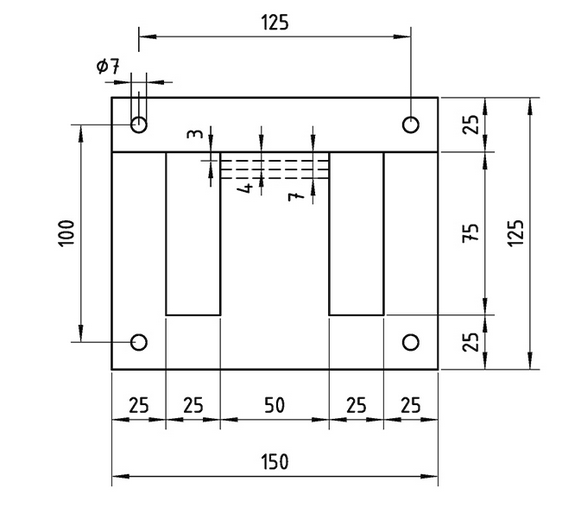
\includegraphics[width=\textwidth]{plano_dimensiones.png}
	\caption{Dimensiones del electroimán [mm].}
	\label{fig:img_plano_dimensiones}
\end{figure}

\noindent El bobinado está conformado por $150$ vueltas de alambre de cobre esmaltado de $2.5\:mm$ de diámetro enrollado alrededor de un carrete de plástico (figura \ref{fig:img_carrete}) que luego se ubica en la rama central de la pieza ``E''.

\begin{figure}[H]
	\centering
	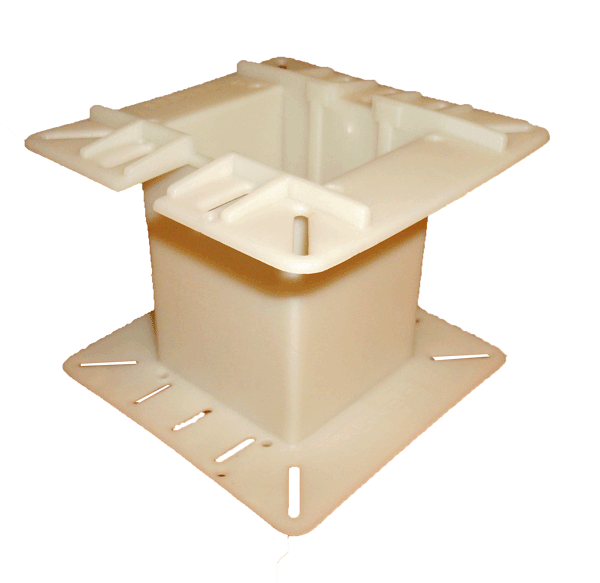
\includegraphics[scale=0.35]{carrete.png}
	\caption{Carrete de plástico para el bobinado.}
	\label{fig:img_carrete}
\end{figure}


\noindent Se utiliza un apilado de láminas cuyo exterior está recubierto por una pintura esmaltada para aislarlas entre sí con el fin de minimizar las pérdidas de energía causadas por las corrientes eléctricas que se generan en el núcleo debidas al flujo magnético. 

\noindent El electroimám está construido por una laminación normalizada sin desperdicio 600. Estas son útiles ya que cada par de laminas ``E'' e ``I'' puede fabricarse a partir de una lámina de acero rectangular, de manera de que no se desperdicia material durante la fabricación. 


%\noindent Está compuesto por dos piezas: una con forma de “E” y otra con forma de “I”. En su núcleo tiene un bobinado de 150 vueltas (N) de cobre esmaltado con un diámetro de $2.5$ mm. El núcleo es de sección cuadrada ya que esto maximiza el área mientras que disminuye el perímetro, reduciendo así la longitud media de las espiras y ahorrando material.

\subsection{Corriente nominal del sistema}

%\noindent Utilizando como referencia la figura \ref{fig:img_dimensiones}, el electroimán del que se dispone tiene las siguientes características:
\noindent Al utilizar los datos de construcción del electroimán mencionados en el apartado \ref{section_caract_constructivas} se puede determinar el valor de corriente necesaria para sostener el objeto del peso deseado.

%\noindent Se debe determinar qué dimensiones debe tener el electroimán a utilizar para que sea capaz de ejercer la fuerza magnética necesaria para mantener levitando el peso deseado.

%\noindent Al analizar la ecuación \ref{eq_fuerza_magnetica} se puede observar que hay dos parámetros que son propios del electroimán: el área del núcleo A y la cantidad de vueltas del bobinado N. 

\noindent Para obtener una expresión de diseño, se parte de la ecuación \ref{eq_fuerza_magnetica} y se iguala a la fuerza ejercida por el peso del objeto que se debe hacer levitar:

\begin{equation}\label{eq_fuerza_peso}
	M*g=\frac{i^{2}*N^{2}*\mu_{o}*A}{4*Y_{g}^{2}}
\end{equation}

\noindent De la ecuación \ref{eq_fuerza_peso} y, a partir de las condiciones de diseño del problema, se puede determinar la corriente necesaria para mantener el objeto en suspensión:

\begin{equation} \label{eq_corriente_peso}
	i_{nom}=\sqrt{\frac{4*M*g*Y_{g}^{2}}{N^{2}*\mu_{o}*A}}
\end{equation}

Si se considera las condiciones mas exigentes para el sistema, con $M=30\:kg$ e $Y_{g}=5\:mm$, se obtiene:

\begin{equation}
	i_{nom}=20.4\:A
\end{equation}

\noindent Si bien esta corriente es suficiente para mantener el objeto en estado de equilibrio, se necesita una corriente mayor para poder responder ante perturbaciones en la distancia de separación. Por lo tanto, se define como corriente máxima: $i_{max}=30\:A$.


\subsection{Expresión de inductancia linealizada}
\label{secc_exp_ind_linealizada}
\noindent A partir de la ecuación \ref{eq_inductancia_vs_y}, se realiza una expansión por serie de Taylor linealizada en torno al punto $Y_{g}=Y_{0}=4\:mm$ y se obtiene:

\begin{equation} \label{eq_inductancia_lineal_teorica}
	L(Y_{g})=-2.2089[\:\frac{H}{m}]*Y_{g}\:[m]+0.0177\:[H]
\end{equation}

\noindent Donde:
\begin{itemize}
	\item $Y_{g}$: distancia del entrehierro en metros [m].
	\item L: inductancia resultante en Henry [H].
\end{itemize}

\section{Mediciones sobre el electroimán}

\noindent Se realizaron mediciones sobre la inductancia y la resistencia interna del electroimán con el objetivo de utilizar los valores obtenidos para el diseño de las demás etapas del sistema.

\subsection{Medición de resistencia del bobinado}

\noindent Para medir la resistencia del bobinado se utilizó una fuente de alimentación de laboratorio y se procedió de la siguiente manera:

\begin{itemize}
	\item Se configuró la fuente para entregar una tensión continua de $5\:V$.
	\item Se configuró la protección de corto circuito en $1\:A$.
	\item Se conectaron los bornes del electroimán a los terminales de la fuente.
	\item Se habilitó la salida de tensión.
	\item Se tomó nota de los valores de tensión y corriente que entregaba la fuente.
\end{itemize}

\noindent Al tener una resistencia serie baja, la fuente de tensión activó la protección de corto circuito de forma tal que la corriente en el electroimán se mantuvo constante en $1\:A$. Al utilizar la medición de tensión entregada por la fuente, cuyo resultado fue de $0.19\:V$, se pudo calcular la resistencia del electroimán mediante la Ley de Ohm:

\begin{equation}
	R_{L}=\frac{V}{I}=\frac{0.19\:V}{1\:A}	\approx0.2\:\Omega
\end{equation}

\subsection{Medición de inductancia}

\noindent Se realizó una caracterización de la inductancia en función del entrehierro. Para hacerlo se utilizó un medidor LCR y láminas de cartón de espesor conocido. La medición consistió en apilar dichas láminas entre ambas piezas del electroimán, donde la suma total de los espesores de las láminas es $Y[mm]$ y luego tomar el valor de inductancia entregado por el medidor $(L(Y_{g})[mH])$. De esta forma, se obtuvieron los siguientes resultados:

\begin{table} [H]
	\begin{center}
		\begin{tabular}{| c | c | c | c | c | c | c | c | c | c |}
			\hline			
			$Y[mm]$ & 0 & 1 & 2 & 3 & 4 & 5 & 6.5 & 8.23 & $\infty$ \\ \hline
			$L(Y_{g})[mH]$ & 76.45 & 33.42 & 22.64 & 18.8 & 16.44 & 14.9 & 14.4 & 12.4 & 8.89\\ \hline
		\end{tabular}
		\caption{Valores de inductancia medidos en función del entrehierro.}
		\label{tab_mediciones_inductancia}
	\end{center}
\end{table}

\noindent Para el caso en que no se utiliza la pieza ``I'', se considera que la distancia es infinita. De esta forma, lo que se mide es la inductancia de dispersión, que son las líneas de campo que se cierran a través del bobinado y no contribuyen a la fuerza magnética para hacer levitar el objeto.



\begin{figure} [H]
	\centering
	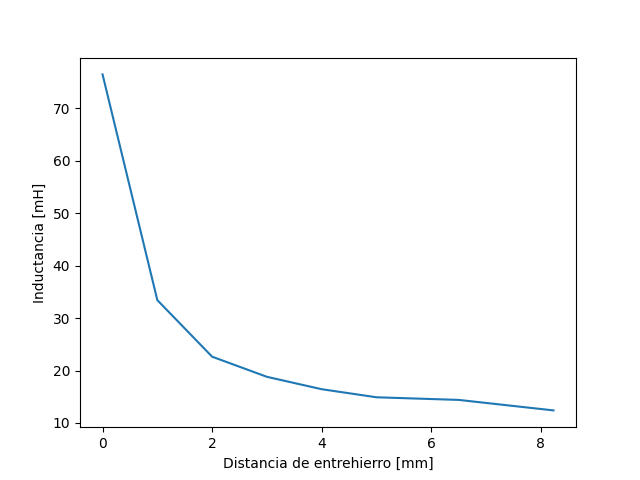
\includegraphics[scale=0.65]{inductancia.png}
	\caption{Inductancia medida en función del entrehierro.}
	\label{fig:img_inductancia_medida}
\end{figure}
\noindent A partir de los resultados mostrados en la tabla \ref{tab_mediciones_inductancia} y en la imagen \ref{fig:img_inductancia_medida} es posible notar que la inductancia no varía linealmente con la distancia. Por lo tanto se realiza una interpolación de primer orden mediante mínimos cuadrados para valores entre $2\:mm$ y $5\:mm$ y se llega a la expresión de inductancia 	\ref{eq_induct_practica}.

\begin{equation}
	\label{eq_induct_practica}
	L(Y_g)=-2.56\:[\frac{H}{m}]*Y_{g}\:[m]+0.027\:[H]
\end{equation}

\noindent Donde:
\begin{itemize}
	\item $Y_{g}$: distancia del entrehierro en metros [m].
	\item L: inductancia resultante en Henry [H].
\end{itemize}

Se puede observar que la expresión obtenida tiene una pendiente similar a la teórica (\ref{eq_inductancia_lineal_teorica}), pero con un valor en el término independiente mayor. Una de las razones de ello es no haber considerado la inductancia de dispersión en el electroimán al momento del modelado. Es decir, no haber tenido en cuenta a las líneas de flujo magnético que se cierran dentro de la pieza en forma de ”E”, y no llegan a atravesar la pieza ”I”.  

Por otro lado, debe tenerse en cuenta que al realizar una aproximación lineal en base a las mediciones, el resultado de la aproximación depende del rango de valores de distancia de entrehierro utilizado para el cálculo. 

La expresión \ref{eq_induct_practica}, obtenida a partir de las mediciones, se acerca más al comportamiento real de la inductancia. Por lo tanto, se utilizará esta expresión para el diseño del resto de las etapas del sistema. 


\section{Modelo de estado de la planta} \label{sec_modelo_estados}

Se desea diseñar un sistema de control que mantenga una levitación de manera estable. Para ello, primero se necesita caracterizar el comportamiento de la planta en función de sus entradas y salidas. Como se analizó en la sección \ref{sec:fuerza_magnetica}, el fenómeno de levitación presenta un comportamiento alineal. Sin embargo, como el sistema va a trabajar en un rango de distancia de entrehierro acotado, su dinámica puede ser aproximada a un comportamiento lineal dentro de ese rango. Esto trae la ventaja de que permite aplicar técnicas de modelado y diseño de compensadores para sistemas lineales.

Una forma de caracterizar la dinámica de un sistema lineal es mediante el modelo de estados. Esto es una representación matemática del comportamiento físico de la planta en función de sus entradas, salidas y variables de estado. Por lo tanto, se decide aplicar este modelo para obtener una función transferencia de la planta que luego será utilizada en el diseño del compensador.

Para obtener este modelo, en primer lugar, se realiza un análisis físico de las fuerzas que gobiernan el movimiento de la pieza ‘’I’’ con el objetivo de llegar a una ecuación diferencial que describa la dinámica del sistema. Para ello, observando la imagen \ref{fig:img_Esquema-del-producto} se plantea la sumatoria de fuerzas:

\begin{equation}\label{eq_sumatoria_fuerzas_y}
	\sum F=M*a=>M*g-F_{m}=M*\ddot{Y_g}
\end{equation}

\noindent Al reemplazar la ecuación \ref{eq_fuerza_magnetica} en la \ref{eq_sumatoria_fuerzas_y} se obtiene:

\begin{equation}\label{eq_sumatoria_fuerzas_y_2}
	\ddot{Y_g}=g-\frac{K}{M}*\frac{i(t)^{2}}{Y_g(t)^{2}}
\end{equation}

\noindent En la expresión \ref{eq_sumatoria_fuerzas_y_2}, K es una constante de valor:

\begin{equation}
	K=\frac{N^{2}*\mu_{o}*A}{4}=1.77*10^{-5} [\frac{N*m^2}{A^2}]
\end{equation}

A partir de la expresión \ref{eq_sumatoria_fuerzas_y_2} se puede obtener un modelo de estados de segundo orden en el que una variable de estado ($x_1$) es la distancia $Y_g$, otra variable ($x_2$) es su derivada (velocidad) y la entrada al sistema (u) es la corriente i. 


\begin{equation*}
	\begin{bmatrix} % El entorno bmatrix puede generar vectores tambien, en ese caso uno de 1 x 3
		&x_{1}=Y_g(t)\\
		&x_{2}=\dot{x_{1}}\\
		&u=i(t)\\
	\end{bmatrix}
\end{equation*}

\noindent Por lo tanto se obtienen dos ecuaciones de estado:

\begin{equation} \label{eq_modelo_estados}
	\begin{bmatrix} % El entorno bmatrix puede generar vectores tambien, en ese caso uno de 1 x 3
		&\dot{x_{1}}\\
		&\dot{x_{2}}\\
	\end{bmatrix}
	=
	\begin{bmatrix} % El entorno bmatrix puede generar vectores tambien, en ese caso uno de 1 x 3
		&f_1(x_1,x_2,u)\\
		&f_2(x_1,x_2,u)\\
	\end{bmatrix}
	=
	\begin{bmatrix} % El entorno bmatrix puede generar vectores tambien, en ese caso uno de 1 x 3
		&x_{2}\\
		&g-\frac{K}{M}*\frac{u^{2}}{x_{1}^{2}}\\
	\end{bmatrix}
\end{equation}

Para obtener un modelo lineal a partir de la expresión \ref{eq_modelo_estados} se utiliza el método de linealización por serie de Taylor en torno al punto de operación de cada variable de estado y entrada al sistema. Este punto de operación se conoce como punto de equilibrio y tiene la particularidad de que ante una entrada constante, las variables de estado también se mantienen constantes, por lo que sus derivadas se anulan. El punto de equilibrio correspondiente a la variable $x_1$ se puede definir como el valor medio del rango de variación de distancia de entrehierro, por lo tanto resulta $x_{1o}=4\:mm$. Los demás puntos de equilibrio se obtienen a partir de resolver el sistema de ecuaciones \ref{eq_puntos_equilibrio}.

\begin{equation} \label{eq_puntos_equilibrio}
	\begin{bmatrix} % El entorno bmatrix puede generar vectores tambien, en ese caso uno de 1 x 3
		&\dot{x_{1}}\\
		&\dot{x_{2}}\\
	\end{bmatrix}
	=
	\begin{bmatrix} % El entorno bmatrix puede generar vectores tambien, en ese caso uno de 1 x 3
		&0\\
		&0\\
	\end{bmatrix}
	=
	\begin{bmatrix} % El entorno bmatrix puede generar vectores tambien, en ese caso uno de 1 x 3
		&x_{2o}\\
		&g-\frac{K}{M}*\frac{u_o^{2}}{x_{1o}^{2}}\\
	\end{bmatrix}
\end{equation}

Finalmente, los puntos de equilibrio del sistema resultan:

\begin{equation}\label{eq_puntos_equil}
	\begin{bmatrix}
		&x_{1o}\\
		&x_{2o}\\
		&u_{o}\\
	\end{bmatrix}
	=
	\begin{bmatrix}
		&4\:mm\\
		&0\\
		&\sqrt{\frac{M*g}{K}}*x_{1o}\\
	\end{bmatrix}
\end{equation}



Como se observa en el sistema de ecuaciones \ref{eq_modelo_estados}, únicamente la función $f_2(x_1,x_2,u)$ es no lineal. Por lo tanto se procede a su linealización en torno a los puntos de equilibrio de la expresión \ref{eq_puntos_equil}. La serie de Taylor desarrollada hasta el factor de primer orden, para un sistema con dos variables de estado y una entrada, queda definida como:

\begin{equation} \label{eq_taylor}
	\dot{x_{2}}=f_2(x_{1o}, x_{2o}, u_{o})+J_1*(x_1-x_{1o})+J_2*(x_2-x_{2o})+J_3*(u-u_o)
\end{equation}

Donde:

\begin{equation} \label{eq_jacobianos}
	\begin{bmatrix} % El entorno bmatrix puede generar vectores tambien, en ese caso uno de 1 x 3
		&{J_{1}}\\
		&{J_{2}}\\
		&{J_{3}}\\
	\end{bmatrix}
	=
	\begin{bmatrix} % El entorno bmatrix puede generar vectores tambien, en ese caso uno de 1 x 3
		&\frac{\partial{f_2(x_1,x_2,u)}}{\partial{x_1}}\Biggr|_{x_{1o},x_{2o},u_o}\\
		&\frac{\partial{f_2(x_1,x_2,u)}}{\partial{x_2}}\Biggr|_{x_{1o},x_{2o},u_o}\\
		&\frac{\partial{f_2(x_1,x_2,u)}}{\partial{u}}\Biggr|_{x_{1o},x_{2o},u_o}\\
	\end{bmatrix}
\end{equation}

Se adoptan nuevas variables de estado equivalentes a las anteriores pero desplazadas por sus puntos de equilibrio:

 \begin{equation*}
 	\begin{bmatrix}
 		&x_1^*\\
 		&x_2^*\\
 		&u^*\\
 	\end{bmatrix}
 	=
 	\begin{bmatrix}
 		&x_1-x_{1o}\\
 		&x_2-x_{2o}\\
 		&u-u_o\\
 	\end{bmatrix}
 \end{equation*}



En la ecuación \ref{eq_taylor}, el primer término correspondiente a la función $f_2(x_{1o},x_{2o},u_o)$ es igual a cero, ya que es la función en el punto de equilibrio. Además, el coeficiente $J_2$ es nulo puesto que la variable $x_2$ no interviene en la función $f_2$. Finalmente el sistema linealizado queda: 


\begin{equation} \label{eq_estados}
	\begin{bmatrix}
		&\dot{x_{1}^*}\\
		&\dot{x_{2}^*}
	\end{bmatrix}
	=
	\begin{bmatrix}
		&x_{2}^*\\
		&2*\frac{K*u_{o}^{2}}{M*x_{1o}^{3}}*x_1^*-2*\frac{K*u_{o}}{M*x_{1o}^{2}}*u^*
	\end{bmatrix}
\end{equation}

Para obtener el modelo de estado se necesitan dos ecuaciones matriciales: la de estados (\ref{eq_estados}) y la de salida. Esta última debe expresarse en función de las variables de estado y de las entradas al sistema. Por lo tanto, se obtiene:

\begin{equation} \label{eq_salida}
	Y=
	\begin{bmatrix}
		&x_{1}^*	
	\end{bmatrix}
\end{equation}

A partir de las expresiones \ref{eq_estados} y \ref{eq_salida} se obtiene el modelo de estado en forma matricial:

\begin{equation*} 
	\begin{bmatrix}
		&\dot{x_{1}^*}\\
		&\dot{x_{2}^*}
	\end{bmatrix}
	=
	A*
	\begin{bmatrix}
		&x_{1}^*\\
		&x_{2}^*
	\end{bmatrix}
	+ B* 
	\begin{bmatrix}		
		&u^*
	\end{bmatrix}
\end{equation*}

\begin{equation*} 
	Y
	=
	C*
	\begin{bmatrix}
		&x_{1}^*\\
		&x_{2}^*
	\end{bmatrix}
	+ D* 
	\begin{bmatrix}		
		&u^*
	\end{bmatrix}
\end{equation*}

\noindent Las matrices del modelo resultan:

\begin{equation*}
	A=
	\begin{bmatrix}
		0 & 1\\
		\frac{2*g}{x_{1o}} & 0
	\end{bmatrix}\\
	  B=
	\begin{bmatrix}
	0\\
	-\frac{2}{x_{1o}}*\sqrt{\frac{K*g}{M}}
	\end{bmatrix}\\
	  C=
	\begin{bmatrix}
	1 & 0\\
	\end{bmatrix}\\
	  D=
	\begin{bmatrix}
	0\\
	\end{bmatrix}\\
\end{equation*}


Con estas matrices se obtiene la función transferencia de la planta que luego será de utilidad para el diseño del compensador. Para obtenerla se utiliza la expresión \ref{eq_transferencia_planta}.

\begin{equation}\label{eq_transferencia_planta}
	G_{P}=C*(s*I-A)^{-1}*B=-\sqrt{\frac{K}{g*M}}*\frac{1}{{(\frac{s}{\sqrt{\frac{2*g}{x_{1o}}}})^2-1}}
\end{equation}

\noindent \noindent Al trabajar con una planta cuya masa es variable es conveniente expresar la transferencia en función de $M$. Finalmente, se obtiene para $x_{1o}=4\:mm$:

\begin{equation} \label{eq_transferencia_planta_m}
	G_{P}(M)=-\sqrt{\frac{30}{M}}*\frac{1.201}{s^{2}-4900}
\end{equation}

\noindent La planta tiene dos polos en $\pm\sqrt{\frac{2*g}{x_{1o}}}=\pm70\:[\frac{rad}{s}]$. Es decir, uno en el semiplano izquierdo y otro en el derecho. Es por este motivo que el fenómeno de levitación magnética es inestable.

\noindent En la expresión \ref{eq_transferencia_planta_m} se observa que la masa del objeto modifica la ganancia del sistema, pero no la ubicación de los polos. Esto es importante para tener en cuenta al momento de diseñar el compensador.

